% =====================================================================================================
% foresight_v4.tex  --  "Could Anyone Have Seen It Coming?"  --  working draft v4  --  2026-07-07
% Rebuild in one step:  python src/build_v4.py   (numbers -> figures -> verify -> latexmk)
% Every number is read from the certified-meter result files; nothing is hand-typed. Provenance:
%   paper/numbers_v4.tex  + gaps_v4/memoir_v4/crossling_v4/exam_v4/circ_v4/duels_v4.tex
%       <- src/make_numbers_v4.py  (checked by src/verify_v4.py, 32/32 re-derivations agree)
%   figures/fig_gaps,fig_memoir,fig_exam,fig_duels.png  <- src/make_figures_v4.py
%   sources: results/{v41_battery,certify_chronicle_heldout,certify_chronicle,v4_battery,v41_defr,
%            certify_defr,diag_*,stats_panel,panel_scores,production_panel}.json
% Supersedes foresight_v3.tex (panel conceptual-strain estimator, retired). v3 files left untouched.
% =====================================================================================================
\documentclass[11pt]{article}
\usepackage[margin=1in]{geometry}
\usepackage[utf8]{inputenc}
\usepackage[T1]{fontenc}
\usepackage{amsmath,amssymb}
\usepackage{graphicx}
\usepackage{booktabs}
\usepackage{caption}
\usepackage{enumitem}
\usepackage[hidelinks]{hyperref}
\usepackage{xcolor}
\usepackage{authblk}
\usepackage[round]{natbib}
\usepackage{appendix}
\captionsetup{font=small,labelfont=bf}
\graphicspath{{../figures/}}
% AUTO-GENERATED by make_numbers_v4.py -- do not edit by hand.
\providecommand{\TBD}{\textbf{[TBD]}}
\newcommand{\NnMeasured}{26}
\newcommand{\NnCovered}{10}
\newcommand{\NnEvents}{8}
\newcommand{\NkaiserPre}{0}
\newcommand{\NkaiserPost}{78}
\newcommand{\NkaiserGap}{+9.84}
\newcommand{\NkaiserPreBets}{Kaiser Wilhelm}
\newcommand{\NkaiserSurpPost}{0.25}
\newcommand{\NkaiserSurpPre}{10.1}
\newcommand{\NkaiserPreImplied}{0.004}
\newcommand{\NkaiserPreBetP}{99}
\newcommand{\NdepBanksMemoir}{94}
\newcommand{\NdepGoldMemoir}{82}
\newcommand{\NnaziDictMemoir}{83}
\newcommand{\NdebtsPre}{80}
\newcommand{\NdebtsPost}{98}
\newcommand{\NdebtsGap}{+0.20}
\newcommand{\NdebtsPreBets}{repudiated by the new rulers}
\newcommand{\NinflendPre}{0}
\newcommand{\NinflendPost}{72}
\newcommand{\NinflendGap}{+6.77}
\newcommand{\NinflendPreBets}{Goldmark}
\newcommand{\NtsarPre}{0}
\newcommand{\NtsarPost}{2}
\newcommand{\NtsarGap}{+2.71}
\newcommand{\NtsarPreBets}{been driven from his throne}
\newcommand{\NusentryPre}{56}
\newcommand{\NusentryPost}{92}
\newcommand{\NusentryGap}{+0.49}
\newcommand{\NusentryPreBets}{the United States}
\newcommand{\NbreadthPre}{99}
\newcommand{\NbreadthPost}{100}
\newcommand{\NbreadthGap}{+0.01}
\newcommand{\NbreadthPreBets}{nearly every great power on earth}
\newcommand{\NpanicsevPre}{97}
\newcommand{\NpanicsevPost}{85}
\newcommand{\NpanicsevGap}{-0.14}
\newcommand{\NpanicsevPreBets}{sharper than any panic in memory}
\newcommand{\NpanicrescPre}{77}
\newcommand{\NpanicrescPost}{79}
\newcommand{\NpanicrescGap}{+0.02}
\newcommand{\NpanicrescPreBets}{Mister Morgan}
\newcommand{\NpanicfirstPre}{5}
\newcommand{\NpanicfirstPost}{13}
\newcommand{\NpanicfirstGap}{+0.92}
\newcommand{\NpanicfirstPreBets}{the national banks}
\newcommand{\NrevrulesPre}{2}
\newcommand{\NrevrulesPost}{4}
\newcommand{\NrevrulesGap}{+0.72}
\newcommand{\NrevrulesPreBets}{the liberals of the parliament}
\newcommand{\NexamTotal}{20}
\newcommand{\NexamAnswered}{16}
\newcommand{\NexamCorrect}{13}
\newcommand{\NexamCorrectPct}{81}
\newcommand{\NexamOutbet}{13}
\newcommand{\NexamOutbetPct}{81}
\newcommand{\NbarAnswer}{14}
\newcommand{\NbarCorrect}{80}
\newcommand{\NbarOutbet}{80}
\newcommand{\NportPre}{5}
\newcommand{\NportPost}{91}
\newcommand{\NportGuess}{Washington}
\newcommand{\NstalinPost}{10}
\newcommand{\NstalinNames}{Trotsky}
\newcommand{\NdevTotal}{20}
\newcommand{\NdevAnswered}{10}
\newcommand{\NfaOld}{41}
\newcommand{\NfaNew}{22}
\newcommand{\NDEexamAnswered}{12}
\newcommand{\NDEexamCorrect}{10}
\newcommand{\NDEexamOutbet}{11}
\newcommand{\NDEexamCovN}{12}
\newcommand{\NFRexamAnswered}{14}
\newcommand{\NFRexamCorrect}{13}
\newcommand{\NFRexamOutbet}{10}
\newcommand{\NFRexamCovN}{14}
\newcommand{\NkaiserENPre}{0}
\newcommand{\NkaiserENPost}{78}
\newcommand{\NkaiserENGap}{+9.8}
\newcommand{\NkaiserENKeeps}{Kaiser Wilhelm}
\newcommand{\NkaiserDEPre}{0}
\newcommand{\NkaiserDEPost}{60}
\newcommand{\NkaiserDEGap}{+13.3}
\newcommand{\NkaiserDEKeeps}{Kaiser Wilhelm}
\newcommand{\NkaiserFRPre}{0}
\newcommand{\NkaiserFRPost}{18}
\newcommand{\NkaiserFRGap}{+5.7}
\newcommand{\NkaiserFRKeeps}{le Kaiser Guillaume}
\newcommand{\NdepFRbets}{repris comme après chaque panique}
\newcommand{\NdepFRp}{98}
\newcommand{\NdepDEbets}{Jahr um Jahr tiefer gesunken}
\newcommand{\NdepDEp}{98}
\newcommand{\NdepENbets}{stood still, neither better nor worse}
\newcommand{\NdepENp}{61}
\newcommand{\NdepENtruthP}{13}
\newcommand{\NtunnelP}{45}
\newcommand{\NpresUncond}{20}
\newcommand{\NpresDefeat}{3}
\newcommand{\NkaiserTwentyNine}{60}
\newcommand{\NmoonNineHundred}{3.58}
\newcommand{\NbreadNineHundred}{4.79}
\newcommand{\NplaneNov}{4.26}
\newcommand{\NplaneFam}{4.29}
\newcommand{\NgasNov}{5.04}
\newcommand{\NgasFam}{4.29}
\newcommand{\NmoneyNov}{4.62}
\newcommand{\NmoneyFam}{4.84}
\newcommand{\NmarkRawTN}{82}
\newcommand{\NmarkRawTh}{31}
\newcommand{\NduelPanicPre}{61}
\newcommand{\NduelNaziPre}{17}
\newcommand{\NduelNaziMargin}{-1.93}
\newcommand{\NduelNaziLawful}{-2.75}
\newcommand{\NduelPanicTrusts}{+2.72}
\newcommand{\NduelFluSerum}{-2.74}
\newcommand{\NfreeTsarTh}{0.67}
\newcommand{\NfreeNaziTN}{0.00}


\title{Could Anyone Have Seen It Coming?\\[2pt]
\large Measuring the Foreseeability of Catastrophe with Minds Frozen in the Past}
\author{Ranke Project}
\date{July 2026 \\[4pt] \small Working draft, v4 --- not for circulation}

\begin{document}
\maketitle

\begin{abstract}
\noindent Were the great catastrophes of the early twentieth century foreseeable before they happened?
The question sits under a large part of economics --- rare-disaster models of the equity premium assume
that investors held, in advance, roughly the disaster probabilities we read off the realized century ---
yet it has never been measured, because every gauge built after the fact already knows the ending. We
build one that does not. Our instrument is a set of language models trained only on text printed before
a fixed year (1900, 1913, or 1929); each is a reader who knows everything published up to its date and
nothing after. We ask such a reader, and a later one who lived through the event, the same question in
the register of a memoir --- ``it is 1919, looking back\ldots'' --- and measure the distance between the
guess of the one and the memory of the other. The instrument is put through an exam of twenty questions
with known answers, passing marks fixed in advance, and certified in English. By this measure some
catastrophes were already in the pre-war picture: the Panic of 1907, the spread of the war to every great
power, the entry of the United States, and --- against the textbook --- the repudiation of Russia's
foreign debts. Others were not: a German republic in place of the Kaiser, the murder of the Tsar, the new
money that ended the inflation. For the Great Depression and Hitler no later reader yet exists; there we
can only read the 1929 mind's memoir of the years ahead, and it reaches for the most recent precedent ---
the Federal Reserve will hold, power will be seized by a march on Berlin, Germany in 1934 will be ruled
by a Wilhelm before a Hitler --- and misses. The disasters were, for the most part, thinkable. What failed
was the weighting: the pre-event mind put its money on the wrong branch of a future it could otherwise
imagine.
\end{abstract}

\section{Introduction}\label{sec:intro}

Ask a well-read German of 1913 who will govern Germany once it has lost a great war, and we can now run
the experiment. A language model trained only on text printed by 1913 --- a reader with everything on the
shelf and nothing after --- is told that the war was lost and asked who stands at the head of the state.
It answers, with near certainty, the Kaiser. A reader frozen sixteen years later, who has read the
newspapers of the republic, answers Ebert. The gap between the two is the object of this paper.

The question is older than the method. Economists model rare disasters as draws from a tail that agents
understand but seldom see: the disaster probabilities that rationalize the equity premium in
\citet{rietz1988} and \citet{barro2006} are read off the realized catastrophes of the twentieth century,
on the assumption that investors attached roughly those probabilities to them beforehand. Historians tell
the opposite story, of catastrophes out of a clear sky --- Europe's statesmen sleepwalking into 1914
\citep{clark2012}, the crash astonishing a nation of optimists \citep{galbraith1955,fisher1930}, Hitler's
chancellorship a bolt from nowhere \citep{turner1996}. Both are claims about a vanished state of knowledge:
what could a contemporary, reading everything in print, have expected? Neither has been tested, because
every measure built after the fact already knows how the story ends. The bond markets of July 1914, which
barely moved until the week the armies marched \citep{ferguson2006}, put the puzzle at its sharpest: was
the war unthinkable, or thinkable and dismissed?

We measure that vanished knowledge directly. Our instrument is a set of language models trained from
scratch on historical text cut off at fixed dates --- 1900, 1913, 1929 --- so that each model is a frozen
reader: everything published up to its year, nothing after. A companion project checked at length that the
models carry no knowledge from after their cutoff, so a frozen reader cannot fake foresight by leaking the
answer. The design turns on a simple contrast. Put a question about the aftermath of a catastrophe to two
readers, one frozen before the event and one frozen after, in the same backward-looking register. For the
later reader the question is history, and it answers from what it read. For the earlier reader the same
question forces an invented memoir of a future it never saw, and what it invents is drawn from its picture
of how the world works. The difference between the guess and the memory is the measurement.

Reaching that design meant discarding two natural alternatives, and the discarding is instructive enough
that Section~\ref{sec:framework} keeps it. A frozen model's surprise at a plain sentence turns out to
measure what its era wrote about, not what its era expected: to the 1900 reader a man walking on the moon
is a smaller surprise than a man buying bread, because moon voyages filled the popular novels and nobody
wrote about buying bread. And a model asked to prophesy --- to complete ``in 1920 the Atlantic will be
crossed by\ldots'' --- answers in the voice of prophecy, which in every library ever assembled belongs to
people who did not know the future. The instrument we keep asks for history instead, and earns trust the
ordinary way, by passing an exam whose questions and passing marks were fixed before it sat down.

Three findings follow. First, most of the catastrophes were thinkable. For the panic, the reach of the
war, the entry of the United States, and the collapse of Russian credit, the pre-event reader's memoir
lands on the truth about as squarely as the memory of a reader who lived through it. The written record of
1913 already held these futures. Second, a few were genuinely outside the picture. That Germany would be a
republic, that the Tsar and his family would be shot, that a wholly new money would end the inflation ---
these the pre-event memoir does not reach, and the size of the miss can be read off in nats. Third, where
no later reader yet exists, for the Depression and for Hitler, the 1929 memoir forecasts by the most recent
precedent and is wrong in a patterned way: the banks will be saved by the new Federal Reserve, the republic
will fall to an armed march as in 1923, the master of Germany will be a Wilhelm. The exceptions to that
rule are the two things its own recent past had taught it --- that a republic can slide into dictatorship,
and that Britain and America can leave gold.

For economics the reading is specific. The support assumption behind the rare-disaster calibrations holds
up well: we find few catastrophes that the pre-event record could not generate, so the ``nobody could
imagine it'' defense of low pre-1914 risk premia is mostly unavailable. The weighting assumption does not:
the same readers put their probability on the wrong branch, and always on the branch the last crisis had
carved. That is the availability heuristic \citep{tversky1973} read out of the written record of an age
rather than a laboratory, and it is the belief distortion that recent theories of credit cycles place at
the center of financial fragility \citep{bordalo2018,gennaioli2018}. The July-1914 bond puzzle then needs
no unthinkability: investors could picture the war; they weighted the wrong future.

The paper also offers a method the text-as-data literature has lacked \citep{gentzkow2019}. Time-locked
readers turn ``what could have been known'' --- the unobservable at the bottom of every argument about
hindsight \citep{kuran1991,tetlock2005,taleb2007} --- into a quantity one can estimate, under stated
conditions and behind an exam that the instrument can fail. Section~\ref{sec:framework} states the question
and why prediction fails. Section~\ref{sec:gap} defines the gap and what it identifies.
Section~\ref{sec:exam} reports the exam that certifies it. Section~\ref{sec:results} gives the
measurements; Section~\ref{sec:memoir} reads the 1929 memoir of the 1930s; Section~\ref{sec:languages}
repeats the exercise in German and French; Section~\ref{sec:limits} says plainly what the instrument cannot
do; Section~\ref{sec:implications} draws out the consequences for disaster-risk models.

\section{The question, and two measures that fail}\label{sec:framework}

Write $\Omega_t$ for what a literate contemporary could read at date $t$: everything in print. A
catastrophe's foreseeability has two parts that ordinary language runs together. One is whether the
outcome was inside the range of futures the worldview could produce at all --- whether it was thinkable.
The other is whether, among the thinkable futures, the worldview put weight on the one that happened. A
peso problem in the exchange-rate sense \citep{krasker1980} is exactly the case where the first holds and
the second fails: the event is conceivable, its probability misjudged. We will measure both. But the two
obvious ways of measuring the first do not work, and it is worth seeing why before building the one that
does.

The first obvious measure is surprise at a sentence. A language model reads a sentence word by word and can
report how probable it found each word; summed, that is a surprise score, low for the familiar and high for
the strange. The natural idea is to score a description of the future under a pre-event reader and call a
high score unforeseeable. It fails on its first test. To the 1900 reader the sentence ``a man walks on the
surface of the moon'' scores \NmoonNineHundred{} per word against ``a man buys bread at the corner shop''
at \NbreadNineHundred{}: the moon is the smaller surprise. The reason is not foresight but print. Jules
Verne's moon voyages had been popular reading since the 1860s, and no one writes a sentence about buying
bread. Averaging twenty different wordings of each idea removes the noise and confirms the verdict: for a
1900 reader, sentences about flying machines score \NplaneNov{} against \NplaneFam{} for motor cars --- no
difference --- even though the motor car was expected and powered flight was not. The one pair that
separates, poison gas at \NgasNov{} against cavalry at \NgasFam{}, separates because poison gas was the
only one of these futures absent from the printed page. Surprise at a sentence measures what an age wrote
about, its stock of images, not what it expected to happen. Appendix~\ref{app:circulation} reports this arm
in full; we keep it as a description of a period's imagination, not of its expectations.

The second obvious measure is to make the model bet on the future. Give it an unfinished sentence in the
future tense and four endings, read off how much probability it puts on each, and treat the money it
withholds from the true ending as its surprise. This fails for a deeper reason. Asked to complete ``in 1920
travellers will cross the Atlantic chiefly by\ldots'', the 1913 reader puts \NtunnelP\% on a tunnel beneath
the sea --- because \emph{Der Tunnel}, a novel about exactly such a tunnel, was a bestseller of 1913.
Worse, the future tense summons the voice of people who do not know the future, which is the only voice
that ever writes in it. Told that Germany has lost the war and asked who will rule, the 1913 reader lowers
its bet on an elected president from \NpresUncond\% to \NpresDefeat\%; a mind that understood the world
would raise it. And the 1929 reader, which has read a decade of newspapers reporting that the Kaiser
abdicated and fled, still bets \NkaiserTwentyNine\% that he rules a defeated Germany --- because asked to
prophesy, it imitates pre-war prophecy rather than reporting what it knows. A forward-framed prompt does
not read the model's knowledge; it reads the genre of prediction. This is the single most important
obstacle in the paper, and the instrument of the next section exists to get around it.

The way around it is to stop asking about the future and ask about the past. History is written backward,
by people who know how it turned out, and a language model has read a great deal of it. So we put every
question in the past tense, as a memoir: not ``Germany will be ruled by'' but ``it is 1919; Germany fought
a great war and was beaten; the head of the state today is''. For the later reader this is a history
question, and history questions reach its knowledge. For the earlier reader it is a request to write a
memoir of a future it never saw --- and the memoir it writes exposes what it genuinely expected, because it
has nothing else to write from. Both readers now speak in the same backward-looking voice, so the
difference between them is no longer voice or style. It is knowledge.

\section{The foresight gap, and what it identifies}\label{sec:gap}

Every question has the same shape: a sentence describing the world just after a catastrophe, four endings,
and two readers. The guesser is frozen before the event; the witness is frozen after. Each reads the same
sentence and assigns the four endings probabilities that add to one --- a betting slip. For the ending that
in fact happened we take each reader's surprise to be minus the logarithm of the probability it placed
there, and define
\[
\text{foresight gap} \;=\; \text{guesser's surprise} - \text{witness's surprise}
\;=\; -\ln p_{\text{guesser}}(\text{truth}) + \ln p_{\text{witness}}(\text{truth}).
\]
A gap near zero, with both readers confident, means the truth was as easy for the one who came before as
for the one who came after: foreseen. A large gap means only the reader who lived through it knows:
unforeseen. The unit is the nat; a gap of about $0.7$ is a factor of two in the odds, a gap of $2$ a factor
of seven.

For the gap to mean foresight and nothing else, three things must hold, and the design is built to secure
each.
\begin{enumerate}[label=(\roman*),leftmargin=2.2em,itemsep=2pt]
\item The witness really knows. The later reader's high bet on the truth has to be knowledge, not luck.
This is what the exam of Section~\ref{sec:exam} tests directly, on questions whose answers we know and
whose witness we can name in advance.
\item The guesser really does not. The earlier reader must carry nothing from after its cutoff, or its low
bet on the truth would understate what a contemporary knew. A companion project checked this at length and
found the models clean of post-cutoff knowledge; a guesser that cannot recall the event cannot be secretly
withholding it.
\item The two are asked alike. Both readers see the same backward-looking sentence and the same four
endings, so the difference between them cannot be register or wording --- both write in the voice of
hindsight. The scoring rule below removes what wording effects remain.
\end{enumerate}

One threat to (iii) is worth naming now, because it also bounds the instrument. These readers retrieve by
fame: shown the true answer beside a more famous rival, a reader can take the celebrity rather than the
truth. The exam will show a clean example. The rule that follows is to ask only where the truth is at least
as famous as its rivals, and to flag any question that breaks it. Section~\ref{sec:limits} returns to this.

The scoring rule secures the tail end of (iii). To keep the mere wording of an ending from deciding the
bet, an early version subtracted from each ending a measure of how common that phrase is in general. That
backfires when the true answer is itself a common phrase. On the question of the mark, the ending ``worth
nothing at all'' is an everyday expression, and the subtraction drove the 1929 reader --- whose own free
writing calls the mark ``worth about one cent'' --- down to zero on it. Scored without the subtraction, the
same reader puts \NmarkRawTN\% there, and the 1913 guesser a sober \NmarkRawTh\%. So we score by two rules.
For endings that are names --- people, places, currencies --- a famous name's commonness is the signal, and
we do not subtract. For endings that are ordinary phrases we compute the bet both ways and keep the
question only if the two agree on the winner; if they disagree the meter declines to answer. A gauge that
sometimes says ``I cannot score this one fairly'' is the price of one that does not mislead.

\section{Certifying the instrument: the exam}\label{sec:exam}

An instrument for a question no one has measured cannot be validated against a known answer to that
question. It can be validated against known answers to questions of the same shape. So before using the
meter we made it sit an exam: twenty questions about events that fall between two model cutoffs, so that for
each one an earlier reader should not know the answer and a later one should. The Panic of 1907 lies after
the 1900 reader's cutoff but before the 1913 reader's, so the 1900 model must guess and the 1913 model
should remember. Three passing marks were written down before anything was run. The meter must agree to
answer at least \NbarAnswer{} of the \NexamTotal{} questions; among those it answers, the witness must name
the true ending at least \NbarCorrect\% of the time; and in at least \NbarOutbet\% it must put more on the
truth than the guesser does, so that knowing more shows. A first run on a separate development set answered
only \NdevAnswered{} of \NdevTotal{} and exposed the scoring flaw of the previous section. We repaired the
scoring, froze every rule, and then ran \NexamTotal{} entirely fresh questions with no further adjustment.
The full exam is Table~\ref{tab:exam}; Figure~\ref{fig:exam} plots it.

\begin{figure}[t]\centering
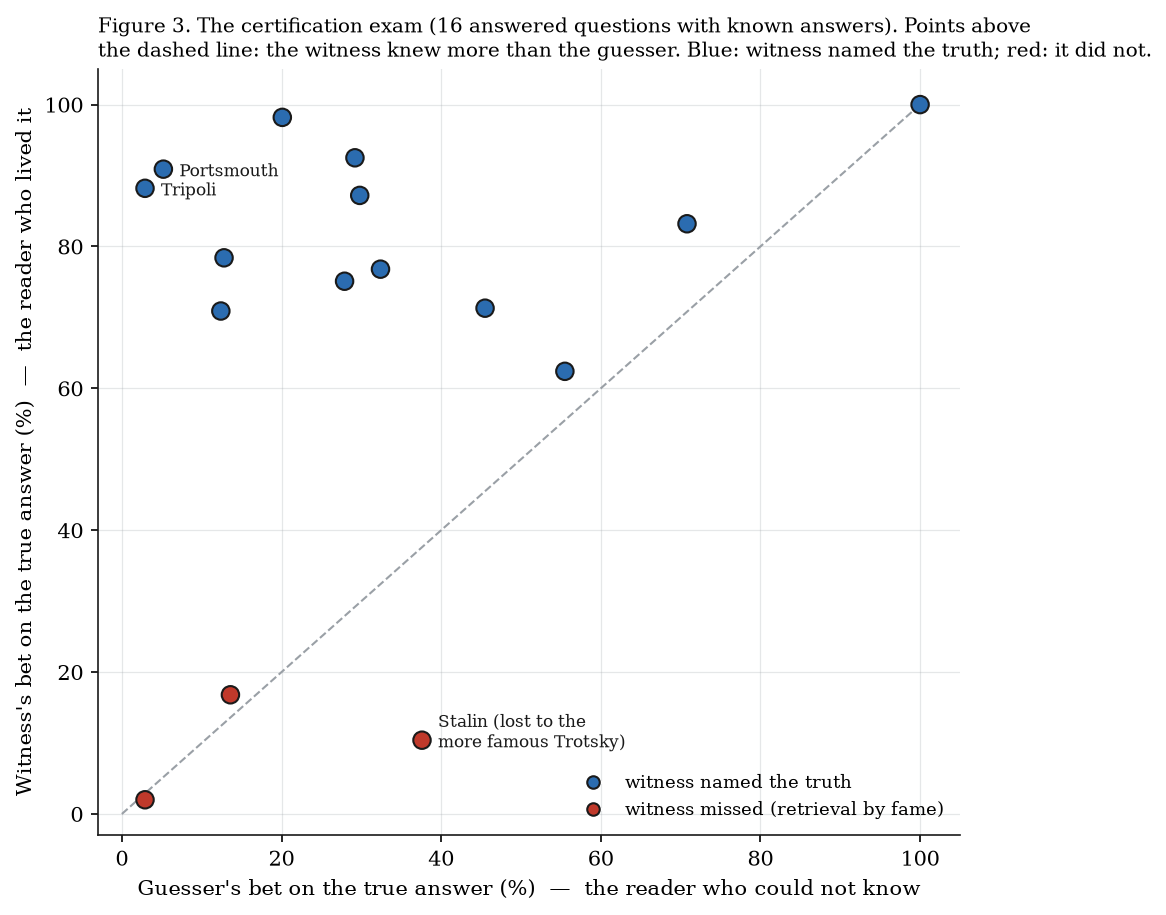
\includegraphics[width=.72\textwidth]{fig_exam.png}
\caption{The certification exam. Each point is one of the \NexamAnswered{} questions the meter agreed to
answer. The horizontal axis shows how much the guesser (the reader who could not know the event) bet on the
true answer; the vertical axis shows how much the witness (the reader who lived through it) bet on the same
answer. Points above the dashed line are questions where the witness knew more than the guesser --- almost
all of them. Blue points are questions where the witness named the truth; the three red points are the
failures, where a more famous rival drew the bet away (Stalin behind Trotsky, Bl\'eriot behind Latham).
Take-away: on questions with known answers, the later reader knows and the earlier reader guesses, which is
what a working instrument must show.}
\label{fig:exam}
\end{figure}

The fresh run passed. Take one question: ``it is 1906; the peace between Russia and Japan was signed last
year at\ldots'', with endings Portsmouth, Washington, Geneva, and The Hague. The 1900 guesser, for whom the
treaty had not happened, put \NportPre\% on Portsmouth and favored \NportGuess{} --- a reasonable guess. The
1913 witness put \NportPost\% on Portsmouth. Across all \NexamTotal{} questions the meter agreed to answer
\NexamAnswered{}, above the mark of \NbarAnswer{}; the witness named the truth in \NexamCorrect{} of those
\NexamAnswered{} ($\NexamCorrectPct\%$, mark \NbarCorrect{}); and the witness out-bet the guesser in
\NexamOutbet{} of \NexamAnswered{} ($\NexamOutbetPct\%$, mark \NbarOutbet{}). All three marks met. The meter
is certified in English.

One failure marks the instrument's limit and is worth keeping in view. Asked who ruled Russia after Lenin's
death, the 1929 reader answered \NstalinNames{}, putting only \NstalinPost\% on Stalin, the right answer. In
the Western press of the late 1920s Trotsky was by far the more written-about man, and these readers
retrieve by fame: set the truth beside a more famous rival and they can take the celebrity. This is the
failure mode of condition (iii), it is real, and it is why we ask only where the truth is the famous
version and flag the questions that break the rule.

That the exam can be failed is the point. The development run did fail it, on coverage, and forced the
scoring repair; the German and French runs fail it too (Section~\ref{sec:languages}). An instrument that
passes an exam it could have failed has earned something a plausible story has not.

\section{What was foreseen, and what was not}\label{sec:results}

We put the certified meter to \NnEvents{} catastrophes between 1907 and 1933, with several questions each.
The meter answered \NnCovered{} of the \NnMeasured{} questions that have a witness; the rest it declined, by
the rule of Section~\ref{sec:gap}. Figure~\ref{fig:gaps} is the paper in one picture, and
Table~\ref{tab:gaps} lists every answered question with its gap.

\begin{figure}[t]\centering
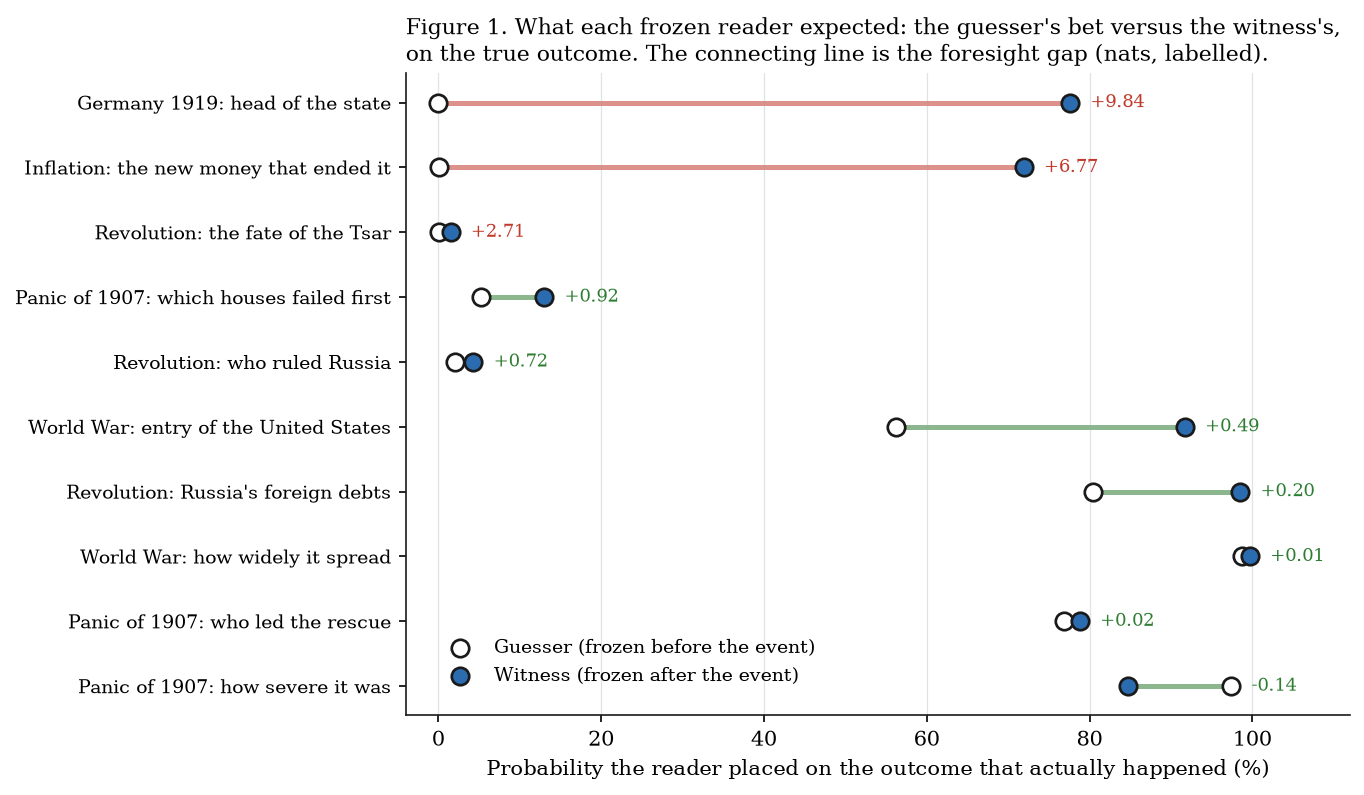
\includegraphics[width=.96\textwidth]{fig_gaps.png}
\caption{The foresight gap, question by question, in English. For each question the open circle is the
guesser's bet on the outcome that in fact happened and the filled circle is the witness's; the horizontal
distance between them, labelled in nats, is the foresight gap. Questions near the top have large gaps: only
the witness knew. Questions near the bottom have small gaps: the earlier reader found the truth about as
easy as the later one. Take-away: the German republic, the new money, and the Tsar's murder were outside the
pre-event picture; the panic, the reach of the war, the entry of the United States, and the collapse of
Russian credit were inside it.}
\label{fig:gaps}
\end{figure}

\begin{table}[t]\centering\small
\begin{tabular}{p{5.3cm}ccr p{3.5cm}}
\toprule
Question & Guesser & Witness & Gap & The guesser's memoir instead \\
\midrule
which houses failed first in the panic of 1907 & 5\% & 13\% & $+0.92$ & the national banks \\
how severe the panic of 1907 was & 97\% & 85\% & $-0.14$ & sharper than any panic in memory \\
who led the rescue in 1907 & 77\% & 79\% & $+0.02$ & Mister Morgan \\
how widely the war spread & 99\% & 100\% & $+0.01$ & nearly every great power on earth \\
who joined the war against Germany in 1917 & 56\% & 92\% & $+0.49$ & the United States \\
what became of Russia's foreign debts & 80\% & 98\% & $+0.20$ & repudiated by the new rulers \\
who ruled Russia after the revolution & 2\% & 4\% & $+0.72$ & the liberals of the parliament \\
what became of the Tsar & 0\% & 2\% & $+2.71$ & been driven from his throne \\
the new money that ended the German inflation & 0\% & 72\% & $+6.77$ & Goldmark \\
who headed the German state in 1919 & 0\% & 78\% & $+9.84$ & Kaiser Wilhelm \\
\bottomrule
\end{tabular}
\caption{The foresight gap, by question, in English. ``Guesser'' and ``witness'' are the probability each
reader placed on the ending that in fact happened; the gap is the guesser's surprise minus the witness's,
in nats. The last column is the ending the guesser's memoir bet on instead. Rows are ordered by gap.}
\label{tab:gaps}
\end{table}

Take the largest gap first, since it is the clearest case. The question is who headed the German state in
1919, with the endings President Ebert, Kaiser Wilhelm, Crown Prince Wilhelm, and Marshal Hindenburg. The
1913 guesser, even after being told the war was lost, put essentially nothing on Ebert --- about
\NkaiserPreImplied\% --- and nearly all of it, \NkaiserPreBetP\%, went wrongly to the Kaiser. The 1929
witness put \NkaiserPost\% on Ebert. The guesser's surprise at the republic is about \NkaiserSurpPre{} nats,
the witness's about \NkaiserSurpPost{}, and the gap between them is \NkaiserGap{} nats, the largest in the
study. A German republic was not in the pre-war picture, not even the picture of a defeated Germany.

The rest of the table sorts into two groups. The foreseen outcomes sit near zero with both readers
confident. The reach of the war to every great power is one (\NbreadthPre\% for the guesser, \NbreadthPost\%
for the witness, gap \NbreadthGap{}); the entry of the United States is another (\NusentryPre\% to
\NusentryPost\%, gap \NusentryGap{}); the severity of the 1907 panic and the identity of its rescuer are two
more --- the 1900 reader already bets on ``Mister Morgan'' to lead the rescue, because a great banker
halting a panic was a familiar American story. That the panic reads as foreseen is not a free pass but a
test the instrument had to clear: financial panics were the one recurring genre in the sample, chosen in
advance as a positive control, and a gauge that made them look like bolts from the blue would have been
wrong. The most surprising of the foreseen is the collapse of Russian credit: asked what became of the
debts Russia owed to France and England, the 1913 guesser put \NdebtsPre\% on ``repudiated by the new
rulers'', against \NdebtsPost\% for the witness, a gap of only \NdebtsGap{}. The ruin of the French
bondholder, so often told as a shock, was fully present in the pre-war mind.

The unforeseen outcomes are few and specific. Besides the republic, there is the fate of the Tsar: the
guesser's memoir has him ``driven from his throne'' with near certainty --- the deposition of 1917 was easy
to foresee, the revolution of 1905 having rehearsed it --- but it does not reach the cellar at
Yekaterinburg, and the murder of the whole family carries a gap of \NtsarGap{} nats. And there is the money
that ended the inflation: the guesser sensibly expects a ``Goldmark'', a gold-backed mark of the old kind,
and is wrong; the Rentenmark, backed by land, was a genuine invention, and the gap is \NinflendGap{} nats.
These are not failures of nerve about how bad things could get. The pre-war reader could imagine a lost war,
a fallen dynasty, a ruined currency. What it could not supply was the particular new thing: a republic, an
execution, a new kind of money.

\section{The memoir of the 1930s}\label{sec:memoir}

For the Great Depression and the Nazi seizure of power no witness model yet exists, because none is trained
past 1929. There is no gap to compute. What we can read is the 1929 reader's memoir of the years just ahead
--- its bets, set beside what happened (Figure~\ref{fig:memoir}, Table~\ref{tab:memoir}).

\begin{figure}[t]\centering
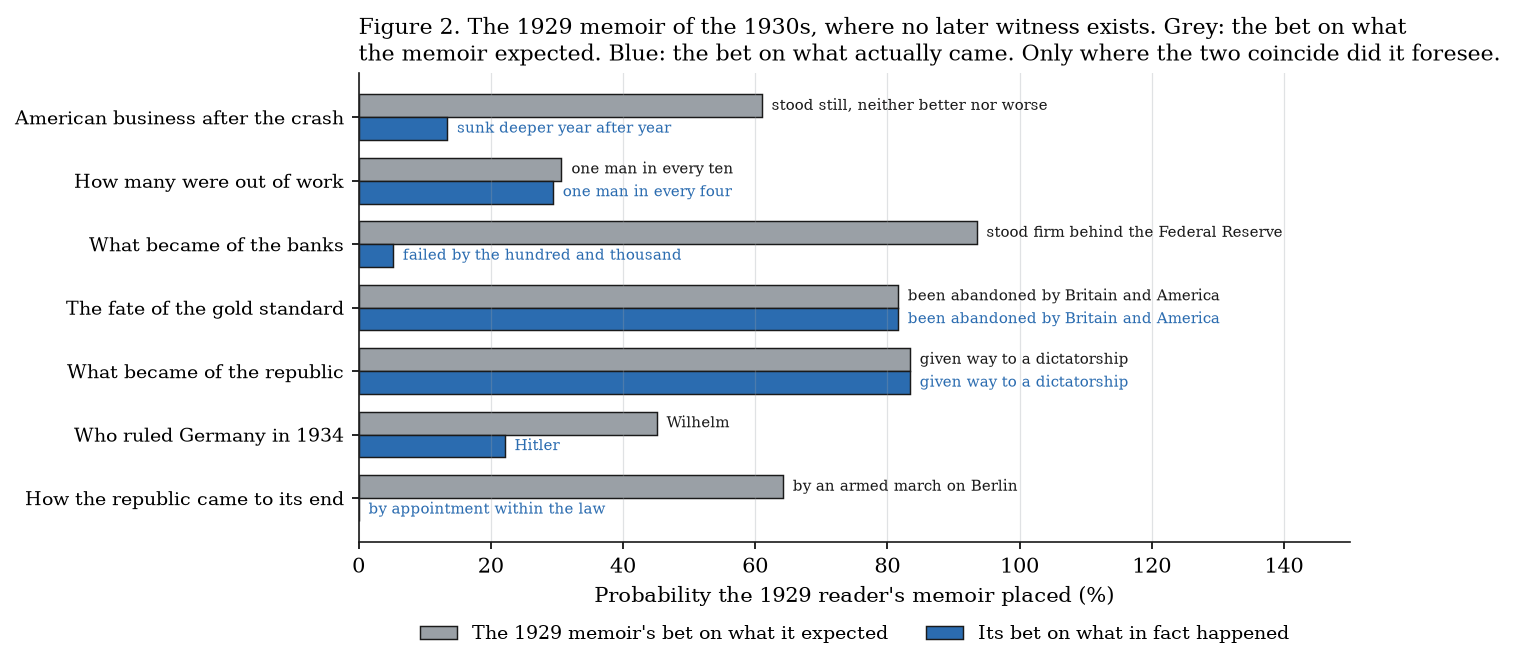
\includegraphics[width=.96\textwidth]{fig_memoir.png}
\caption{The 1929 reader's memoir of the 1930s, where no later witness exists. For each question the grey
bar is how much the memoir bet on the future it expected, the blue bar how much it bet on the future that
actually came; the text on each bar names the outcome. Where the two bars line up (the gold standard, the
slide into dictatorship) the memoir foresaw; where the grey bar towers over the blue (the course of
business, the fate of the banks, the ruler, the path to power) it expected the wrong thing. Take-away: the
misses are all the most recent precedent, reapplied.}
\label{fig:memoir}
\end{figure}

\begin{table}[t]\centering\small
\begin{tabular}{p{4.6cm}p{4.1cm}cp{3.5cm}c}
\toprule
Question & The 1929 memoir expects & Its bet & What in fact happened & Its bet on that \\
\midrule
the course of American business after the crash & stood still, neither better nor worse & 61\% & sunk deeper year after year & 13\% \\
how many Americans were out of work & one man in every ten & 31\% & one man in every four & 29\% \\
what became of America's banks & stood firm behind the Federal Reserve & 94\% & failed by the hundred and thousand & 5\% \\
the fate of the gold standard & been abandoned by Britain and America & 82\% & been abandoned by Britain and America & 82\% \\
what became of the Weimar republic & given way to a dictatorship & 83\% & given way to a dictatorship & 83\% \\
who ruled Germany in 1934 & Wilhelm & 45\% & Hitler & 22\% \\
how the republic came to its end & by an armed march on Berlin & 64\% & by appointment within the law & 0\% \\
\bottomrule
\end{tabular}
\caption{The 1929 reader's memoir of the 1930s. No later reader exists, so there is no gap --- only the 1929
guesser's bets, beside the outcome that in fact followed and the bet the guesser placed on it.}
\label{tab:memoir}
\end{table}

The misses share one shape: the most recent precedent, applied again. American business, the memoir
expects, will have ``\NdepENbets'' four years after the crash ($\NdepENp\%$), the ordinary end of an
ordinary panic; in fact it sank deeper year on year, an ending the memoir gives \NdepENtruthP\%. The banks
will ``stand firm behind the Federal Reserve'', the new institution of 1913, trusted at \NdepBanksMemoir\%;
in fact they failed by the thousand. Power in Germany will be seized by an armed march on Berlin --- the
Kapp putsch of 1920, the Munich putsch of 1923, replayed --- and the master of Germany in 1934 will be a
Wilhelm before a Hitler. Each guess is the last crisis, reached for again.

Two bets land, and they are the two things the 1929 reader's own recent past had taught it. It expects the
Weimar republic to give way to a dictatorship (\NnaziDictMemoir\%), because its newspapers were already full
of government by emergency decree. And it finds it entirely likely that Britain and America will leave the
gold standard (\NdepGoldMemoir\%), because it had lived through exactly that between 1914 and 1925. Where the
future rhymed with the reader's own experience, the memoir was right; where the future broke new ground, it
reached for the nearest old thing.

\begin{quote}\small
A false alarm, caught by the rules. An earlier version of the ruler question seemed to have the 1929 memoir
putting \NfaOld\% on ``the leader of the National Socialists'' governing Germany in 1934 --- striking
foresight for 1929, when that party polled under three per cent. Rewritten with bare names --- Hitler,
Hindenburg, Wilhelm, Ludendorff --- the bet on Hitler falls to \NfaNew\%, no better than chance, and the
memoir's favorite is Wilhelm. The apparent foresight was the fluency of a stock phrase, not knowledge, and
it is exactly the error the two-rule scoring and the exam exist to catch.
\end{quote}

\section{The same test in German and French}\label{sec:languages}

The models read German and French as well as English, so we translated the exam and all the catastrophe
questions and ran the whole exercise again in each language, under the same rules and the same passing
marks. The instrument does not clear the bar in either. German answered only \NDEexamAnswered{} of
\NexamTotal{} exam questions --- below the mark of \NbarAnswer{} --- though where it did answer it was right
\NDEexamCorrect{} times out of \NDEexamAnswered{}: precise, but too often silent, which is a fault of our
German answer wording rather than of the meter. French answered \NFRexamAnswered{} and was right
\NFRexamCorrect{} times, but the witness out-bet the guesser in only \NFRexamOutbet{} of \NFRexamAnswered{},
short of the third mark, and it fell short mostly on questions where the guesser was already right for good
reason --- women's suffrage, or a King George who in 1900 already reigned in Greece. So the headline claims
rest on English; the other two languages are supporting evidence, reported as such, and we do not adjust the
marks to let them pass.

They support the central result. The question of who headed Germany in 1919 is answered in all three
languages, and the answer is the same everywhere (Table~\ref{tab:crossling}): the guesser keeps the Kaiser,
the witness names Ebert, and the gap is large in every language.

\begin{table}[t]\centering\small
\begin{tabular}{lccr p{3.2cm}}
\toprule
Language & Guesser & Witness & Gap & The guesser's memoir keeps \\
\midrule
English & 0\% & 78\% & $+9.8$ & Kaiser Wilhelm \\
German & 0\% & 60\% & $+13.3$ & Kaiser Wilhelm \\
French & 0\% & 18\% & $+5.7$ & le Kaiser Guillaume \\
\bottomrule
\end{tabular}
\caption{The flagship question in three languages. The guesser's bet on the republic, the witness's bet, and
the gap in nats. The guesser keeps a monarch in every language; the gap is the German republic's distance
from the pre-war picture, and it is large everywhere.}
\label{tab:crossling}
\end{table}

The three languages also show something no single one could. Asked how American business fared in the four
years after the crash, the French memoir bets \NdepFRp\% on \emph{\NdepFRbets} --- recovered, as after every
panic --- while the German memoir bets \NdepDEp\% on \emph{\NdepDEbets} --- sunk deeper year on year. The
German memoir is the one that gets it right, and the likely reason is memory: the German 1920s, with their
inflation and slumps, had taught the German-language press what a collapse can be, while the French press
remembered recoveries. Each language forecasts from its own national memory. No survey taken in 1929 could
have recovered that.

\section{What the instrument cannot do}\label{sec:limits}

Four limits bound the claims, and we state them rather than bury them.

First, coverage is partial by design. The meter answered \NnCovered{} of the \NnMeasured{} questions with a
witness and declined the rest, because the two scoring rules disagreed on them. Refusal is a feature --- it
is what keeps the meter from scoring questions where wording, not knowledge, would decide --- but it means
the results describe the questions the meter could score, not a random sample of all questions. We read the
answered set, not a census.

Second, retrieval by fame is a real failure mode, not a hypothetical one. The exam caught it (Stalin behind
Trotsky), and it would bias any question that set the truth beside a more famous rival. We ask only where
the truth is the famous version and flag the exceptions, but the reader should treat a small gap on a
fame-loaded question with the same caution we do.

Third, the two post-1929 events have no witness. The Depression and the Nazi seizure are read only as the
1929 memoir, with no later reader to anchor the gap, so for them we report the guesser's bets beside history
and claim no measured gap. A reader trained to 1938 would close this, and is the obvious next step.

Fourth, only English is certified. German and French fail the exam as it stands --- German on coverage,
French on the third mark --- so their agreement with the English result is supporting evidence, not
independent confirmation. Better-worded answer options in those languages are needed before their numbers
can carry weight of their own.

None of these overturns the central reading, because that reading rests on English questions the meter
answered and the exam certified. But each marks a place where the instrument is still short of what one
would want, and where more work would sharpen it.

\section{What the measurements change}\label{sec:implications}

Return to \citet{barro2006}. The rare-disaster account of the equity premium reads a disaster probability
off the realized twentieth century and attributes it, before the fact, to investors. Our measurements speak
to both halves of that move. On the first half the calibrations come off well. We find few catastrophes ---
not the war, not the fall of the empires, not the entry of the United States, not even the repudiation of
Russian debt --- that the pre-event record could not generate. The defense of low pre-1914 risk premia that
rests on unthinkability is mostly not available, and on this the calibrations are vindicated against their
historian critics. On the second half they are not. The same readers put their probability on the wrong
branch of the futures they could imagine, and always on the branch the last crisis had carved: cholera for
the next plague, a putsch for the next seizure of power, a gold-backed mark for the next stable money.
Support was wide; the weighting was biased toward the most recent precedent.

That distinction has a price tag. A gap of two nats is a factor of seven in the odds, and gaps of that size
are what we measure on the outcomes that broke with precedent. The July-1914 bond puzzle \citep{ferguson2006}
then needs no appeal to the unimaginable: investors could picture the war --- its spread, its length, its
draw on the whole world are all in the pre-war reader's memoir --- but they weighted the wrong future.
Models of time-varying disaster premia \citep{gabaix2012,wachter2013} acquire a state variable that can be
read decade by decade: perceived tail risk should load on how recent and how vivid the last precedent was,
and time-locked readers make that loading measurable. For the peso-problem tradition \citep{krasker1980} the
method supplies the missing observable, the state that is in minds but not in samples, read out of the minds
directly.

The reading also reaches the economics of beliefs. Diagnostic-expectations theory
\citep{bordalo2018,gennaioli2018} was built on laboratory work \citep{tversky1973} and tested on modern
credit-cycle data. The duels of Appendix~\ref{app:selection} supply something that literature has lacked:
the same memory-driven bias governing the tail beliefs of a whole society, a century before the surveys,
with the distorting precedent named event by event. Belief formation by availability is not a modern
artifact of financial markets; it is how the written record itself weighed the future.

\section{Conclusion}\label{sec:conclusion}

Foreseeability can be measured, once you build a gauge that does not already know the ending. Frozen
readers, asked for memoirs rather than prophecies and checked against an exam, give one number per
catastrophe: how much harder the truth was for the mind that came before than for the mind that came after.
By that number, most of the early twentieth century's disasters were thinkable in advance --- the panic, the
reach and length of the war, the fall of the dynasties, the ruin of Russian credit read, to the readers of
1900 and 1913, about as easily as they read to a reader who lived through them. A few were not: a republic
in Germany, the murder of the Tsar, a new kind of money. And where no later reader yet exists, the 1929 mind
forecasts the 1930s by its own most recent crisis and misses, except where the future happened to rhyme with
its past. The failure of the age was less one of imagination than of weighting --- and, we now find, that
failure was regular enough to measure. A reader trained to 1938 would let us measure the last two directly,
and turn the memoir of the 1930s from a description into a number.

\begin{thebibliography}{99}
\bibitem[Angell(1910)]{angell1910} Angell, Norman. 1910. \emph{The Great Illusion}. London: Heinemann.
\bibitem[Barro(2006)]{barro2006} Barro, Robert J. 2006. ``Rare Disasters and Asset Markets in the Twentieth
Century.'' \emph{Quarterly Journal of Economics} 121(3): 823--866.
\bibitem[Barro and Urs\'ua(2008)]{barroursua2008} Barro, Robert J., and Jos\'e F. Urs\'ua. 2008.
``Macroeconomic Crises since 1870.'' \emph{Brookings Papers on Economic Activity} 39(1): 255--350.
\bibitem[Bloch(1899)]{bloch1899} Bloch, Ivan S. 1899. \emph{Is War Now Impossible?} London: Grant Richards.
\bibitem[Bordalo et al.(2018)]{bordalo2018} Bordalo, Pedro, Nicola Gennaioli, and Andrei Shleifer. 2018.
``Diagnostic Expectations and Credit Cycles.'' \emph{Journal of Finance} 73(1): 199--227.
\bibitem[Bruner and Carr(2007)]{bruner2007} Bruner, Robert F., and Sean D. Carr. 2007. \emph{The Panic of
1907}. Hoboken: Wiley.
\bibitem[Clark(2012)]{clark2012} Clark, Christopher. 2012. \emph{The Sleepwalkers: How Europe Went to War in
1914}. London: Allen Lane.
\bibitem[Evans(2003)]{evans2003} Evans, Richard J. 2003. \emph{The Coming of the Third Reich}. London: Allen
Lane.
\bibitem[Ferguson(2006)]{ferguson2006} Ferguson, Niall. 2006. ``Political Risk and the International Bond
Market between the 1848 Revolution and the Outbreak of the First World War.'' \emph{Economic History Review}
59(1): 70--112.
\bibitem[Fisher(1930)]{fisher1930} Fisher, Irving. 1930. \emph{The Stock Market Crash---and After}. New
York: Macmillan.
\bibitem[Gabaix(2012)]{gabaix2012} Gabaix, Xavier. 2012. ``Variable Rare Disasters: An Exactly Solved
Framework for Ten Puzzles in Macro-Finance.'' \emph{Quarterly Journal of Economics} 127(2): 645--700.
\bibitem[Galbraith(1955)]{galbraith1955} Galbraith, John Kenneth. 1955. \emph{The Great Crash, 1929}.
Boston: Houghton Mifflin.
\bibitem[Gennaioli and Shleifer(2018)]{gennaioli2018} Gennaioli, Nicola, and Andrei Shleifer. 2018. \emph{A
Crisis of Beliefs: Investor Psychology and Financial Fragility}. Princeton: Princeton University Press.
\bibitem[Gentzkow et al.(2019)]{gentzkow2019} Gentzkow, Matthew, Bryan Kelly, and Matt Taddy. 2019. ``Text
as Data.'' \emph{Journal of Economic Literature} 57(3): 535--574.
\bibitem[Keynes(1919)]{keynes1919} Keynes, John Maynard. 1919. \emph{The Economic Consequences of the
Peace}. London: Macmillan.
\bibitem[Krasker(1980)]{krasker1980} Krasker, William S. 1980. ``The `Peso Problem' in Testing the
Efficiency of Forward Exchange Markets.'' \emph{Journal of Monetary Economics} 6(2): 269--276.
\bibitem[Kuran(1991)]{kuran1991} Kuran, Timur. 1991. ``Now Out of Never: The Element of Surprise in the East
European Revolution of 1989.'' \emph{World Politics} 44(1): 7--48.
\bibitem[Rietz(1988)]{rietz1988} Rietz, Thomas A. 1988. ``The Equity Risk Premium: A Solution.''
\emph{Journal of Monetary Economics} 22(1): 117--131.
\bibitem[Taleb(2007)]{taleb2007} Taleb, Nassim Nicholas. 2007. \emph{The Black Swan}. New York: Random House.
\bibitem[Tetlock(2005)]{tetlock2005} Tetlock, Philip E. 2005. \emph{Expert Political Judgment}. Princeton:
Princeton University Press.
\bibitem[Turner(1996)]{turner1996} Turner, Henry Ashby. 1996. \emph{Hitler's Thirty Days to Power: January
1933}. Reading, MA: Addison-Wesley.
\bibitem[Tversky and Kahneman(1973)]{tversky1973} Tversky, Amos, and Daniel Kahneman. 1973. ``Availability:
A Heuristic for Judging Frequency and Probability.'' \emph{Cognitive Psychology} 5(2): 207--232.
\bibitem[Wachter(2013)]{wachter2013} Wachter, Jessica A. 2013. ``Can Time-Varying Risk of Rare Disasters
Explain Aggregate Stock Market Volatility?'' \emph{Journal of Finance} 68(3): 987--1035.
\bibitem[Zweig(1942)]{zweig1942} Zweig, Stefan. 1942. \emph{The World of Yesterday}. Stockholm:
Bermann-Fischer.
\end{thebibliography}

\clearpage
\appendix
\renewcommand{\thesection}{\Alph{section}}

\section{The exam in full}\label{app:exam}
Table~\ref{tab:exam} lists all \NexamTotal{} held-out questions. For each, ``guesser'' is the probability
the reader frozen before the event placed on the true answer, ``witness'' the probability the reader frozen
after placed on it. ``Answered'' records whether the two scoring rules agreed enough for the meter to score
the question; ``witness right'' whether the witness named the truth. The English run met all three
pre-registered marks: \NexamAnswered{} answered (mark \NbarAnswer{}), witness right in $\NexamCorrectPct\%$
of answered (mark \NbarCorrect{}), witness out-bets the guesser in $\NexamOutbetPct\%$ (mark \NbarOutbet{}).
Every prompt and every ending is in \texttt{results/certify\_chronicle\_heldout.json}; the development run
that set the scoring rule is in \texttt{results/certify\_chronicle.json}.

\begin{table}[h]\centering\small
\begin{tabular}{p{6.6cm}cccc}
\toprule
Question & Guesser & Witness & Answered? & Witness right? \\
\midrule
The decisive sea battle of the Russo-Japanese war & 14\% & 17\% & yes & no \\
Where the Russo-Japanese peace was signed (1905) & 5\% & 91\% & yes & yes \\
Who succeeded to the British throne (1910) & 71\% & 83\% & yes & yes \\
The warship that renamed a class (1906) & 29\% & 92\% & yes & yes \\
Who first flew across the Channel (1909) & 3\% & 2\% & yes & no \\
The country of the 1908 revolution & 56\% & 62\% & yes & yes \\
Who seized Tripoli from the Ottomans (1911) & 3\% & 88\% & yes & yes \\
The isthmus the canal finally crossed & 12\% & 53\% & declined & -- \\
The form China took after 1911 & 12\% & 71\% & yes & yes \\
The fortress of the great 1916 battle & 32\% & 77\% & yes & yes \\
The largest naval battle of the war (1916) & 13\% & 78\% & yes & yes \\
The month the war ended (1918) & 28\% & 75\% & yes & yes \\
The town of the 1925 treaty & 30\% & 87\% & yes & yes \\
Who named the 1924 reparations plan & 20\% & 98\% & yes & yes \\
Who ruled Russia after Lenin & 38\% & 10\% & yes & no \\
The city of the 1921--22 naval conference & 46\% & 71\% & yes & yes \\
What became of Germany's colonies & 0\% & 32\% & declined & -- \\
What Austria became after 1918 & 18\% & 23\% & declined & -- \\
The fate of the surrendered German fleet & 3\% & 1\% & declined & -- \\
What women won after the war & 100\% & 100\% & yes & yes \\
\bottomrule
\end{tabular}
\caption{The held-out certification exam, all \NexamTotal{} questions. Guesser and witness are the bets on
the true answer; a question is ``declined'' when the two scoring rules disagree on the winner.}
\label{tab:exam}
\end{table}

\section{The circulation arm: surprise at a sentence}\label{app:circulation}
This arm measures what a period wrote about, not what it expected, and is reported so the reader can see why
we do not use it for foresight. For each idea we scored twenty wordings under the pre-event reader and
averaged (Table~\ref{tab:circ}). Two of the three pairs show no difference between the expected future and
the unexpected one; the pair that separates, poison gas against cavalry, does so because poison gas was the
one future absent from print. A frozen reader's surprise at a sentence is a reading of an age's stock of
images. It is a real quantity, and it is not a measure of expectation.

\begin{table}[h]\centering\small
\begin{tabular}{llrr l}
\toprule
Pair & Unexpected idea & \multicolumn{1}{c}{Its score} & \multicolumn{1}{c}{Expected idea's} & Verdict \\
\midrule
flying machines vs motor cars & flying machines & 4.26 & 4.29 & no difference \\
poison gas vs cavalry charges & poison gas & 5.04 & 4.29 & clearly apart \\
money made worthless vs a state gone bankrupt & money made worthless & 4.62 & 4.84 & no difference \\
\bottomrule
\end{tabular}
\caption{Surprise at a sentence, 1900 reader, twenty wordings per idea, in nats per word. Lower means less
surprising. Where the expected and unexpected futures score alike, the measure is reading what was printed,
not what was expected.}
\label{tab:circ}
\end{table}

\section{The selection arm: a forced choice between true and false}\label{app:selection}
The gap of the main text measures whether the truth was reachable. This arm asks a narrower question within
a single reader: shown the outcome that happened and an equally dramatic one that did not, which does the
reader prefer? Because the two options are matched for drama, wording largely cancels, and the preference
reads which future the record favored. Figure~\ref{fig:duels} and Table~\ref{tab:duels} give the share of
such pairs each reader gets right. The pattern is the one the main text names: the readers beat a coin where
catastrophe was a familiar genre --- the 1900 reader takes the true anatomy of the coming panic in
\NduelPanicPre\% of pairs --- and fall below it where the event broke with precedent. The 1929 reader takes
the true path to the Nazi seizure in only \NduelNaziPre\% of pairs, betting against lawful appointment and
for the armed march (margin \NduelNaziLawful{} nats). Free generation tells the same story: prompted for the
aftermath of a lost war, the 1913 reader volunteers the Tsar's deposition in a fraction \NfreeTsarTh{} of
completions, but no reader ever volunteers the corporal as master of Germany (\NfreeNaziTN). One caution:
several duels, chiefly for the war and the empires, pit the truth against a counterfactual that shares the
event's own language, so they carry little information by construction; the informative duels are the panic,
the pandemic, and the Nazi seizure. This arm supports the weighting story of
Section~\ref{sec:implications}; it does not, on its own, measure foreseeability.

\begin{figure}[h]\centering
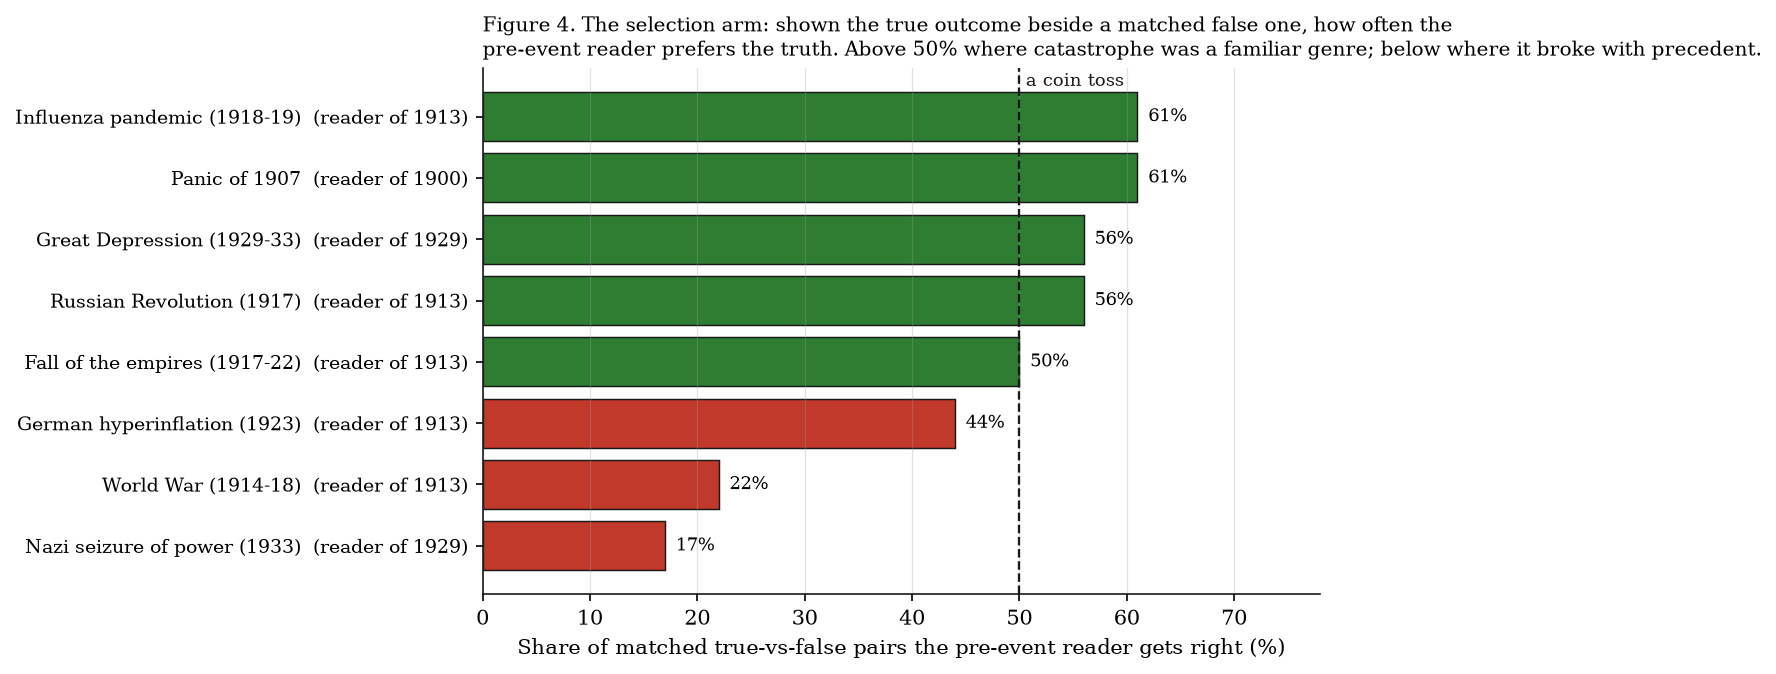
\includegraphics[width=.92\textwidth]{fig_duels.png}
\caption{The selection arm. For each event, the share of matched true-versus-false pairs the pre-event reader
gets right, pooled over the three languages; fifty per cent is a coin. Green above the line, red below.
Take-away: the pre-event reader beats the coin where catastrophe was a recurring genre and falls below it
where the event broke with precedent.}
\label{fig:duels}
\end{figure}

\begin{table}[h]\centering\small
\begin{tabular}{lrrrr}
\toprule
Event & Reader 1900 & 1913 & 1929 & Modern \\
\midrule
Nazi seizure of power (1933) & 28\% & 33\% & 17\% & 33\% \\
Panic of 1907 & 61\% & 61\% & 56\% & 50\% \\
Influenza pandemic (1918-19) & 61\% & 61\% & 44\% & 50\% \\
World War (1914-18) & 33\% & 22\% & 33\% & 28\% \\
Fall of the empires (1917-22) & 50\% & 50\% & 39\% & 39\% \\
Great Depression (1929-33) & 56\% & 50\% & 56\% & 50\% \\
Russian Revolution (1917) & 44\% & 56\% & 56\% & 39\% \\
German hyperinflation (1923) & 50\% & 44\% & 44\% & 50\% \\
\bottomrule
\end{tabular}
\caption{Forced choice between the true outcome and a matched false one: share of pairs each reader gets
right, pooled over the three languages, by event. Fifty per cent is a coin.}
\label{tab:duels}
\end{table}

\section{German and French exams}\label{app:defr}
Neither language clears the bar, and the shortfalls are informative. German answered \NDEexamAnswered{} of
\NexamTotal{} (below the mark of \NbarAnswer{}) but was right \NDEexamCorrect{} of \NDEexamAnswered{} where
it answered: the problem is our German answer wording, which draws too many refusals, not the meter's
precision. French answered \NFRexamAnswered{} and was right \NFRexamCorrect{}, but the witness out-bet the
guesser in only \NFRexamOutbet{} of \NFRexamAnswered{}, and the misses are questions where the guesser was
already right for good reason. We report English as certified and the other two as supporting evidence, and
we do not retrofit the marks. Full per-question results are in \texttt{results/certify\_defr.json} and
\texttt{results/v41\_defr.json}.

\section{Abandoned designs}\label{app:graveyard}
For the record, the approaches tried and dropped, each reproducible from the results files. Surprise at a
sentence, kept as the circulation arm above, was dropped as a foresight measure once the moon scored below
bread. Averaging twenty wordings removed the noise and confirmed the null rather than rescuing it. Betting
in the future tense was dropped when the 1913 reader bet on a transatlantic tunnel and the 1929 reader, told
of the defeat, still bet on the Kaiser. Scoring only by the popularity-subtracted rule was dropped because
it drove common-phrase truths to zero; scoring only by the raw rule was dropped because it let stock phrases
win whether true or not; the two-rule agreement test is what remained. An earlier cross-model comparison
that differenced a frozen reader against a modern one was withdrawn when it proved to measure the gap between
model families rather than the gap in knowledge. The diagnostic files are
\texttt{results/diag\_square\_one.json}, \texttt{diag\_paraphrase\_pilot.json},
\texttt{diag\_betting\_pilot.json}, \texttt{diag\_retro\_pilot.json}, and \texttt{diag\_retro\_v2.json}.

\end{document}
